\subsection{About ARFC}
\begin{frame}
  \frametitle{Advanced Reactors and Fuel Cycles group (PI: Kathryn Huff)}
               \begin{figure}[t]
                \vspace*{-0.1in}
                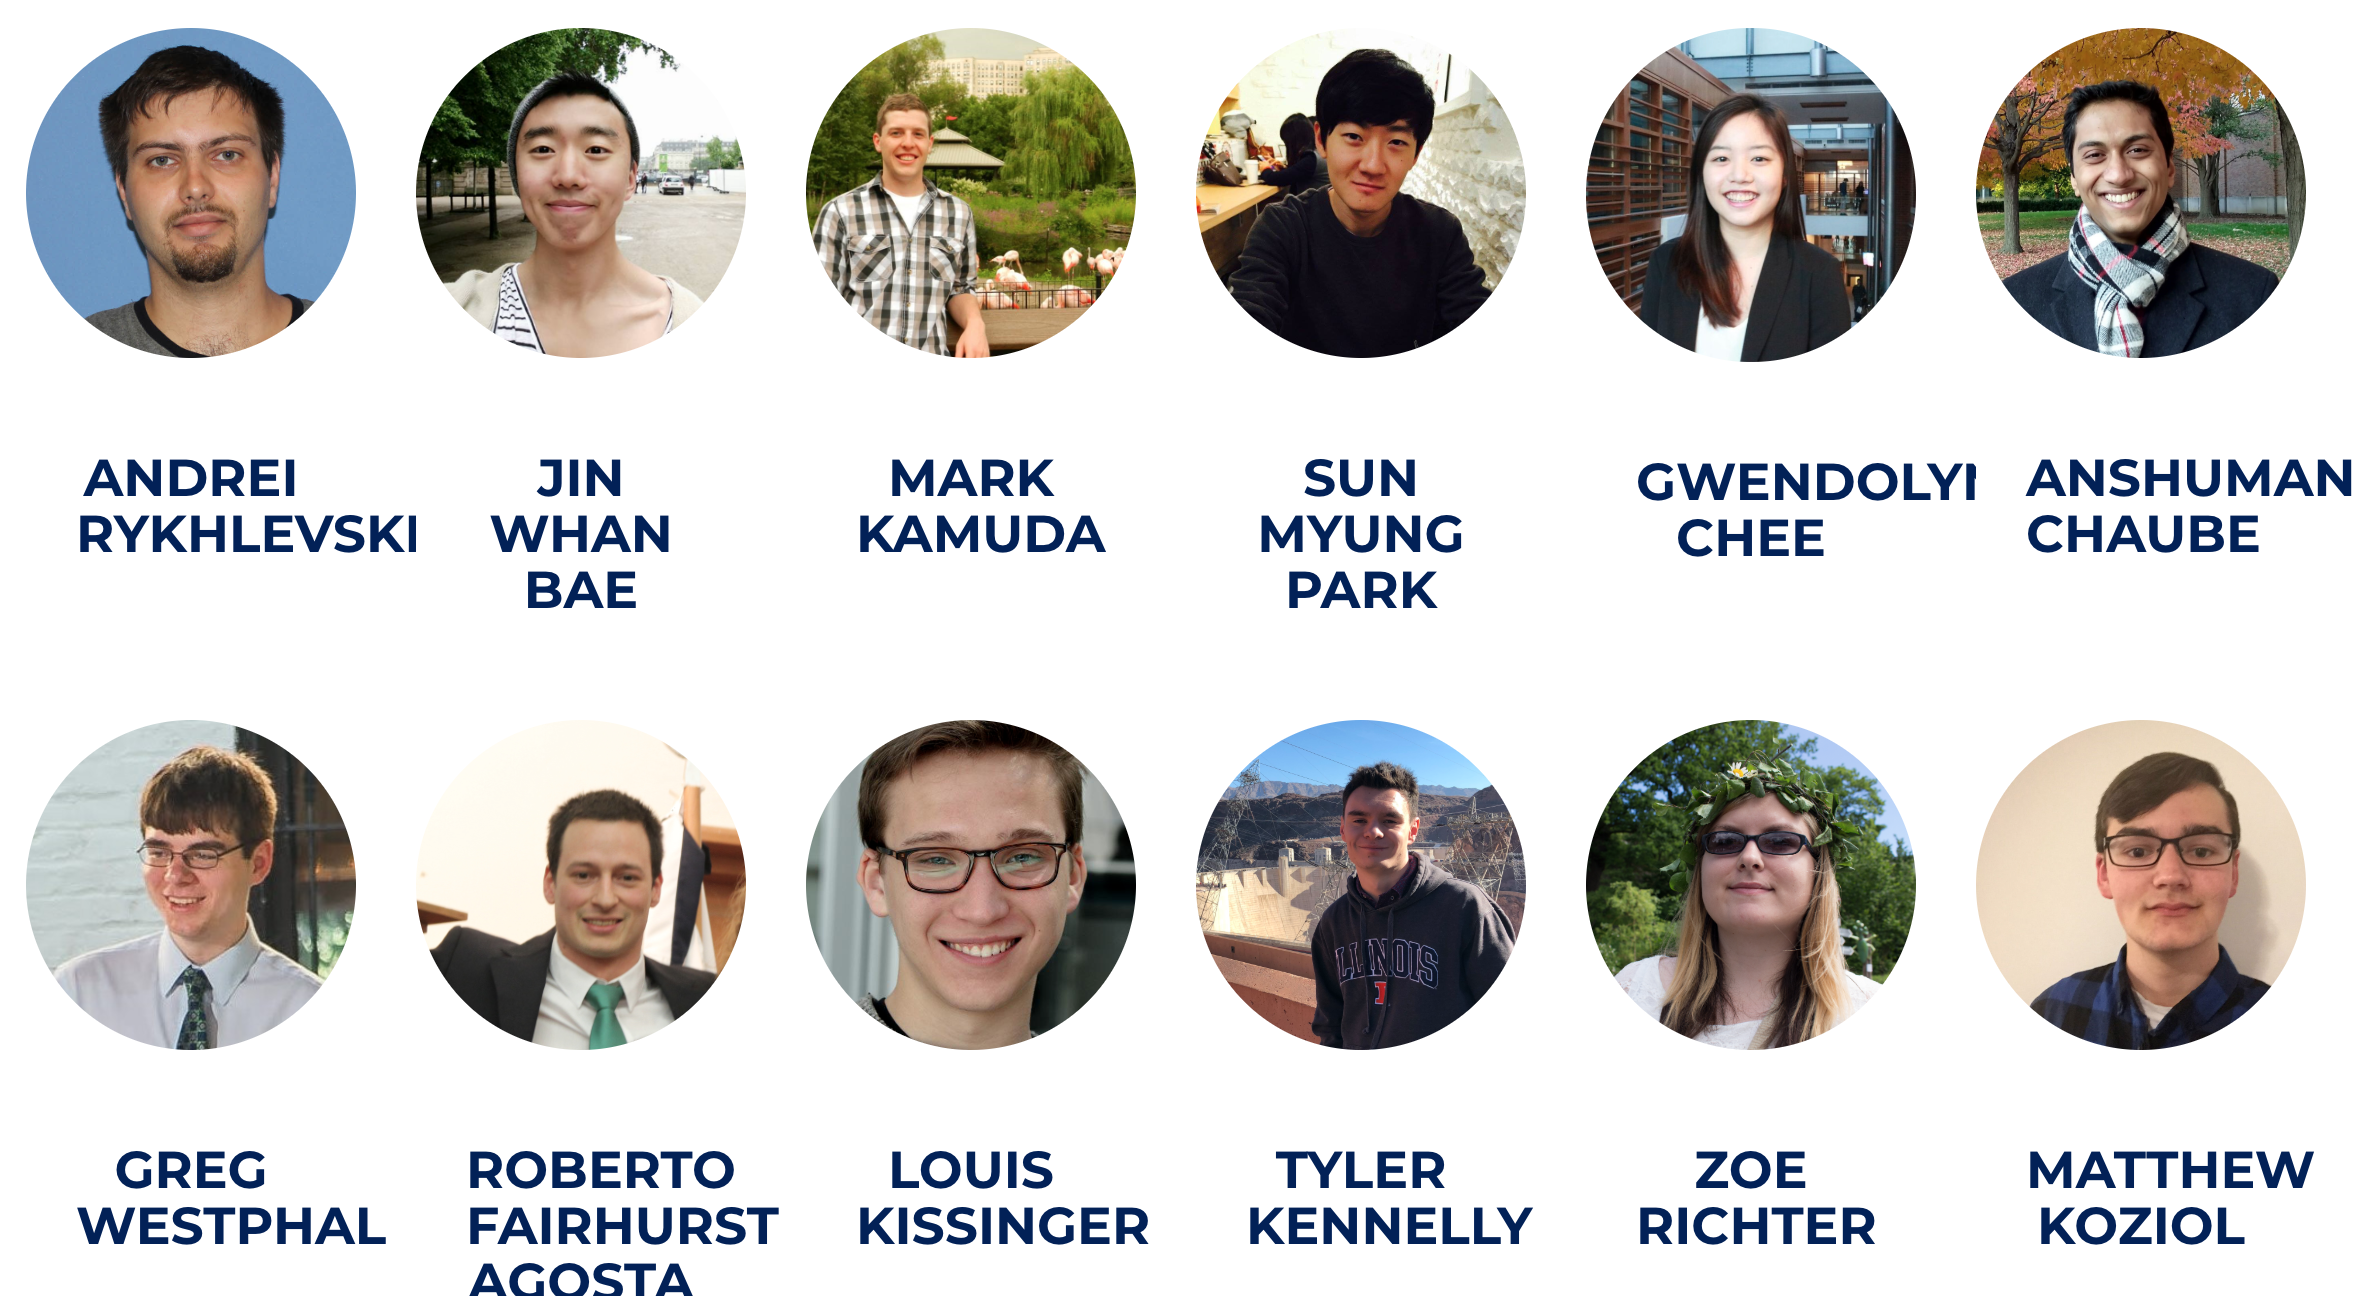
\includegraphics[height=0.71\textwidth]{./images/arfc1.png}
               \end{figure}            
\end{frame}

\begin{frame}
  \frametitle{Insights at Disparate Scales}
               \begin{figure}[t]
                \vspace*{-0.1in}
			\hspace*{-0.35in}
                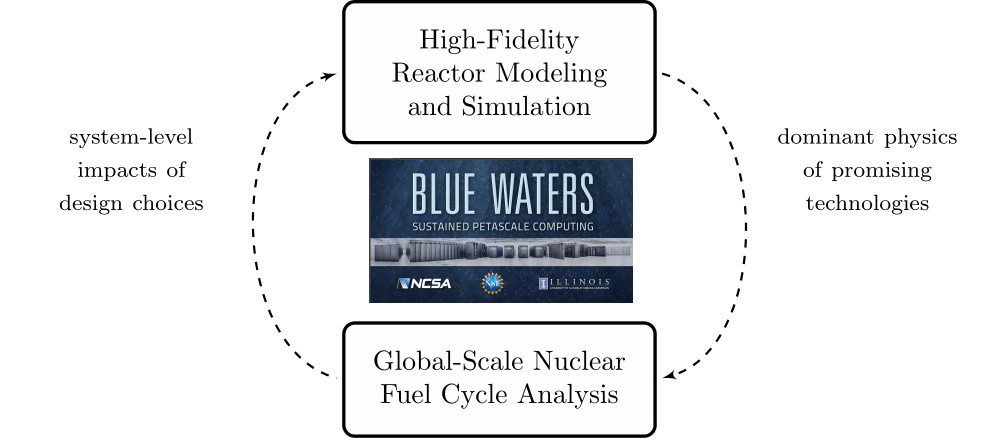
\includegraphics[height=0.5\textwidth]{./images/synergy.png}
               \end{figure}            
\end{frame}

\subsection{Fission basics}
\begin{frame}
  \frametitle{Nuclear Fission Reaction}
               \begin{figure}[t]
                \vspace*{-0.1in}
			\hspace*{-0.35in}
                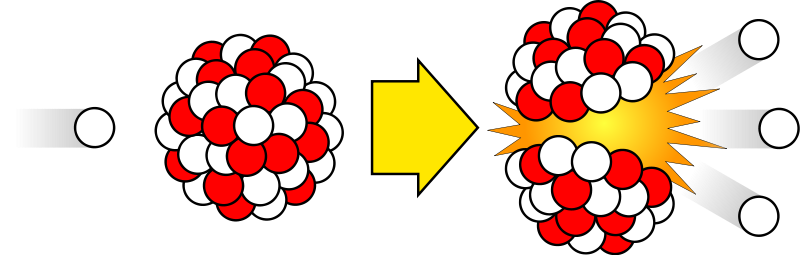
\includegraphics[height=0.25\textwidth]{./images/800px-Fission.png}
               \end{figure}            
\end{frame}

\begin{frame}
  \frametitle{Nuclear Fission Chain Reaction}
               \begin{figure}[t]
                \vspace*{-0.1in}
			\hspace*{-0.35in}
                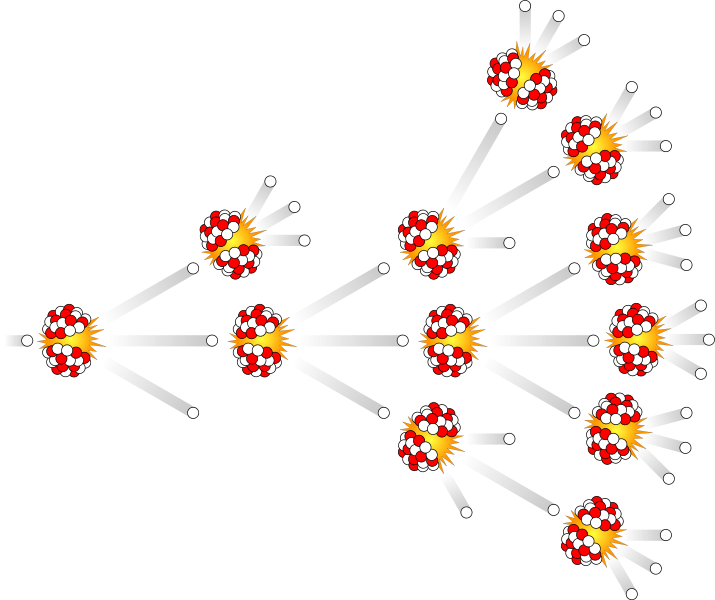
\includegraphics[height=0.7\textwidth]{./images/715px-Chainreaction.png}
               \end{figure}            
\end{frame}

\begin{frame}
  \frametitle{Nuclear Power Plant}
  \animategraphics[width=\textwidth,autoplay,loop]{6}{./images/gif/frame-}{0}{23}
\end{frame}

\subsection{Motivation}
\begin{frame}
  \frametitle{Why Molten Salt Reactors?}
                  \vspace*{-0.1in}
              \begin{block}{Main advantages of liquid-fueled \glspl{MSR} \cite{elsheikh_safety_2013}}
               \begin{enumerate}
                \item High coolant temperature (600-750$^{\circ}$C).
                \item Various fuels can be used ($^{235}$U, $^{233}$U, Thorium, U/Pu).
                \item Increased inherent safety.
                \item High fuel utilization $\Rightarrow$ less nuclear waste generated.
                \item Online reprocessing and refueling.
               \end{enumerate}
               \end{block}
                  \vspace*{-0.1in}               
               \begin{block}{Main advantages of \gls{MSBR} \cite{robertson_conceptual_1971}}
               \begin{enumerate}
                \item Produces more fissile material than it consumes (breeding ratio 1.06).
                \item Thorium cycle limits plutonium and minor actinides.
                \item Could transmute spent fuel from existing \gls{NPP}.
               \end{enumerate}
               \end{block}

\end{frame}

\begin{frame}
  \frametitle{Challenges in simulation \gls{MSR}}
                  \vspace*{-0.05in}
               \begin{enumerate}
                \item Contemporary burnup codes cannot treat fuel movement.
                \item Neutron precursor location is hard to estimate.
                \item Operational and safety parameters change during reactor operation.
                \item Power generation strongly depends on fuel temperature and vica versa.
               \end{enumerate}

           \begin{figure}[t]
                \vspace*{-0.05in}
			\hspace*{-0.2in}
                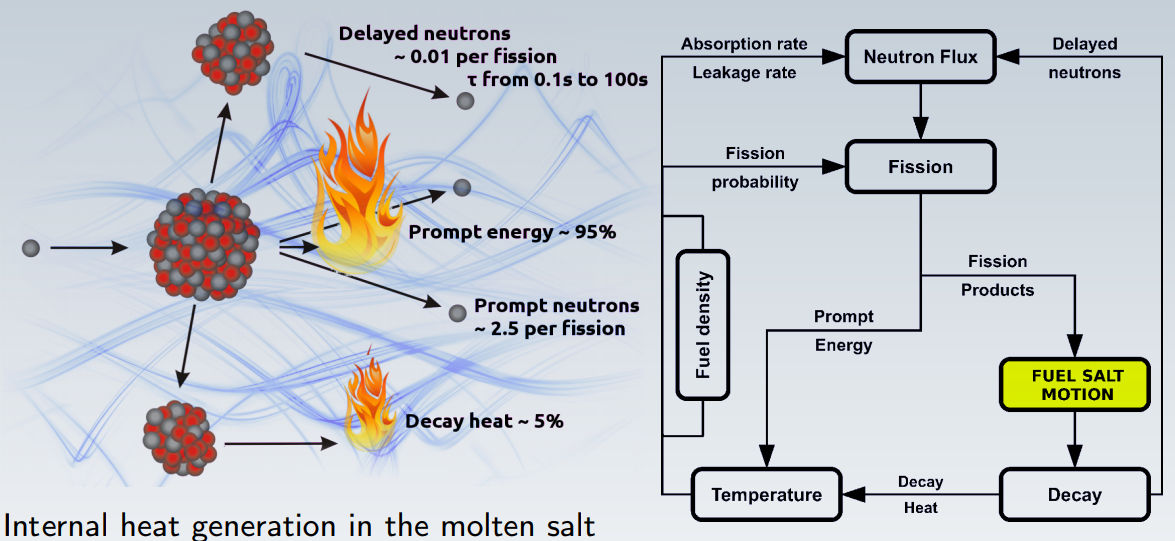
\includegraphics[height=0.47\textwidth]{./images/coupled_physics.png}
		\vspace*{-0.05in}
		\caption{Challenges in simulating \gls{MSR} (Courtesy of Manuele Aufiero,2012).}
     	 \end{figure}               
\end{frame}

\begin{frame}
  \frametitle{Research objectives}
                  \vspace*{-0.1in}
              \begin{block}{Goal \#1: Tool for online reprocessing depletion simulation (SaltProc)\cite{rykhlevskii_saltproc}}
               \begin{enumerate}
                \item Create high-fidelity full-core neutronics model of MSBR.
                \item Develop online reprocessing simulation code, SaltProc, which expands the neutronics code capability for simulation liquid-fueled \gls{MSR} operation.
                \item Analyse \gls{MSBR} neutronics and fuel cycle performance.
               \end{enumerate}
               \end{block}

              \begin{block}{Goal \#2: Tool for multiphysics simulation of \gls{MSR} (Moltres)\cite{lindsay_introduction_2018}}
               \begin{enumerate}
                \item Demonstrate steady-state coupling of neutron fluxes, precursors, and thermal-hydraulics.
                \item Implement advective movement of delayed neutron precursors.
                \item Demonstrate capabilities with 2D axisymmetric and 3D mesh.
               \end{enumerate}
               \end{block}


              
\end{frame}
